  % !TEX root = main.tex
% -----------------------------------------------------------------------------
% Experiments Chapter Template
% Private Query Refinement
% -----------------------------------------------------------------------------

\section{Experiments}
\label{sec:experiments}

This section presents the experimental evaluation of our private query-refinement
explanation framework. The goal of the evaluation is to study both the efficiency
and the quality of the proposed method under different datasets, query pairs,
privacy budgets, and algorithmic parameters.

\subsection{Experimental Goals}
\label{subsec:experimental-goals}

The experiments are designed to answer the following research questions:

\begin{description}
    \item[RQ1 -- Scalability.]
    How does the running time of the proposed algorithm scale with the database
    size, number of predicates, number of released explanations, privacy budget,
    and view-selection parameter?

    \item[RQ2 -- Utility.]
    How useful are the released explanations compared with non-private and
    brute-force baselines?

    \item[RQ3 -- Privacy impact.]
    How does the privacy budget $\epsilon$ affect the quality and stability of
    the selected explanations and released histograms?

    \item[RQ4 -- Case-study interpretability.]
    Do the explanations reveal meaningful semantic differences between the
    original query and the refined query in realistic analysis scenarios?
\end{description}

% TODO: Add a short paragraph connecting these questions to the problem definition
% and algorithmic contributions from Sections~\ref{sec:model} and~\ref{sec:algorithm}.

\subsection{Experimental Setup}
\label{subsec:experimental-setup}


\subsubsection{Datasets}

\paragraph{IPUMS-CPS.}
We use a down-sampled version of the IPUMS-CPS dataset containing
\textbf{100,000} tuples.

\paragraph{Stack Overflow Developer Survey.}
We also evaluate the method on the Stack Overflow Developer Survey dataset.

\paragraph{Hospital Dataset.}
To evaluate the framework in the context of consistent query answering (CQA),
we use the Hospital dataset commonly used in prior repair and data-cleaning
work \cite{rekatsinas2017}.

The dataset contains hospital records with attributes such as:
\[
\texttt{HospitalName},\ \texttt{City},\ \texttt{State},
\texttt{ZipCode},\ \texttt{PhoneNumber},\ \texttt{HospitalType}.
\]

The dataset contains inconsistencies with respect to functional dependencies:
\[
\texttt{HospitalName} \rightarrow \texttt{ZipCode},
\]
\[
\texttt{HospitalName} \rightarrow \texttt{PhoneNumber},
\]
and:
\[
\texttt{ZipCode} \rightarrow \texttt{City}.
\]

\subsubsection{Query Pairs}
Table~\ref{tab:query-pairs} summarizes the planned query pairs and the
attributes used for explanations.

\begin{table*}[t]
\centering
\caption{Query pairs used in the experiments.}
\label{tab:query-pairs}
\begin{tabular}{p{0.12\linewidth} p{0.28\linewidth} p{0.28\linewidth} p{0.18\linewidth}}
\toprule
\textbf{Dataset} & \textbf{$Q_1$} & \textbf{$Q_2$} & \textbf{Semantic difference} \\
\midrule
IPUMS-CPS &
\texttt{EMPSTAT = Employed AND UHRSWORK >= 35} &
\texttt{EMPSTAT = Employed AND UHRSWORK < 35} &
Full-time vs. part-time employment \\

IPUMS-CPS &
\texttt{EMPSTAT = Employed AND EDUC >= Bachelor's degree} &
\texttt{EMPSTAT = Employed AND EDUC < Bachelor's degree} &
Employed people with vs. without higher education \\

IPUMS-CPS &
\texttt{EMPSTAT = Employed AND INCTOT >= 60000} &
\texttt{EMPSTAT = Employed AND INCTOT < 30000} &
High-income vs. low-income employed people \\

Stack Overflow &
\texttt{YearsCodePro >= 10} &
\texttt{YearsCodePro < 4} &
Professional vs. early-career developers \\

Stack Overflow &
\texttt{WorkRemote = Fully remote} &
\texttt{WorkRemote = On-site} &
Remote vs. on-site workers \\

Stack Overflow &
\texttt{JobSat > 5 AND UsingAI = Yes} &
\texttt{JobSat > 5 AND UsingAI = No} &
Satisfied developers using vs. not using AI tools \\
\bottomrule
\end{tabular}
\end{table*}

% TODO: Add exact executable query syntax from the codebase.
% TODO: Add the explanation attributes for each query pair, for example:
% IPUMS-CPS: UHRSWORK, SEX, AGE, EDUC, INCTOT, RACE.
% Stack Overflow: DevType, LanguageHaveWorkedWith, YearsCodePro, Country, CompanySize.


Unless stated otherwise, we use the following default configuration:
\[
    k = 3, \qquad \tau = 50, \qquad \epsilon = 1,
\]
where $k$ is the number of explanations to release, $\tau$ is the number of views
selected by the private usefulness filter, and $\epsilon$ is the total privacy
budget.

The predicate space consists of all conjunctions of the form
\[
    A_1 = v_1 \wedge A_2 = v_2,
\]
where $A_1,A_2$ are attributes and $v_1,v_2$ are values from their corresponding
domains.

% TODO: Confirm whether single-attribute predicates are also included.
% TODO: Confirm whether numeric attributes are bucketized before predicate generation.
% TODO: Add the number of trials. Planned default: 10 trials.

\subsection{Compared Methods}
\label{subsec:compared-methods}

We compare the following methods.

\begin{description}
    \item[Private-Explanations.]
    The proposed differentially private algorithm. It first privately selects
    useful views, then privately selects the top-$k$ explanations using the
    exponential mechanism, and finally releases noisy histograms.

    \item[Brute-Force.]
    A non-private baseline that evaluates the same predicate space and selects
    the highest-scoring explanations without privacy noise.

    \item[Brute-Force with Non-Proxy Utility.]
    A non-private baseline that directly evaluates the original utility function
    rather than the proxy quality function used by the private algorithm.
\end{description}

% TODO: Add exact implementation details for each baseline.
% TODO: Clarify whether the baselines use the same filtered predicate space or all predicates.

\subsection{Scalability Experiments}
\label{subsec:scalability}

The scalability evaluation measures the running time of the algorithms under
controlled changes to a single parameter while keeping all other parameters fixed
at their default values.

\subsubsection{Varying Dataset Size}
\label{subsubsec:runtime-tuples}

We measure running time as a function of the number of tuples by down-sampling
the input dataset.

\paragraph{Protocol.}
For each dataset size $n \in \{\texttt{TODO}\}$, we sample $n$ tuples from the
full dataset and run each method for $10$ trials.

\paragraph{Expected plot.}
Figure~\ref{fig:runtime-tuples} reports running time as a function of $n$.

\begin{figure}[t]
    \centering
    % \includegraphics[width=0.9\linewidth]{figures/runtime_by_tuples.pdf}
    \fbox{\parbox{0.85\linewidth}{\centering TODO: Runtime vs. number of tuples}}
    \caption{Running time as a function of the number of tuples.}
    \label{fig:runtime-tuples}
\end{figure}

\subsubsection{Varying the Algorithm}
\label{subsubsec:runtime-algorithm}

We compare the running time of Private-Explanations, Brute-Force, and Brute-Force
with Non-Proxy Utility.

% TODO: Add plot and discussion.

\subsubsection{Varying $k$}
\label{subsubsec:runtime-k}

We measure running time as a function of the number of explanations $k$.

\[
    k \in \{\texttt{TODO: e.g., 1, 2, 3, 5, 10}\}.
\]

% TODO: Add plot and discussion.

\subsubsection{Varying the Number of Predicates}
\label{subsubsec:runtime-predicates}

We measure running time as a function of the size of the predicate space.

% TODO: Define how predicate subsets are generated.
% TODO: Add plot and discussion.

\subsubsection{Varying $\epsilon$}
\label{subsubsec:runtime-epsilon}

We measure running time as a function of the privacy budget $\epsilon$.
Although $\epsilon$ primarily affects the randomness of private selection and the
scale of Laplace noise, this experiment verifies whether the implementation has
any budget-dependent runtime overhead.

\[
    \epsilon \in \{\texttt{TODO: e.g., 0.1, 0.25, 0.5, 1, 2, 5}\}.
\]

% TODO: Add plot and discussion.

\subsubsection{Varying $\tau$}
\label{subsubsec:runtime-tau}

We measure running time as a function of the number of views selected by the
private usefulness filter.

\[
    \tau \in \{\texttt{TODO: e.g., 10, 25, 50, 100, 200}\}.
\]

% TODO: Add plot and discussion.

\subsection{Case Studies}
\label{subsec:case-studies}

The case studies evaluate whether the output histograms provide meaningful
interpretations of the semantic difference between the two queries.

For each dataset and query pair, we generate heatmaps of the released histograms
under different settings:

\begin{itemize}
    \item initial predicate set;
    \item $\tau$;
    \item algorithm type, to study the impact of privacy;
    \item $\epsilon$, to study the impact of the privacy budget.
\end{itemize}

Each heatmap has explanation attributes on one axis and selected predicates or
attribute values on the other axis. The cell values represent the noisy histogram
counts or normalized differences released by the algorithm.

% TODO: Decide whether heatmap cells contain raw noisy counts, normalized noisy
% counts, or differences between Q and Q'.

\begin{figure}[t]
    \centering
    % \includegraphics[width=0.9\linewidth]{figures/case_study_heatmap.pdf}
    \fbox{\parbox{0.85\linewidth}{\centering TODO: Case-study heatmap}}
    \caption{Example heatmap of released explanation histograms.}
    \label{fig:case-study-heatmap}
\end{figure}

\subsubsection{IPUMS-CPS Case Study}
\label{subsubsec:ipums-case-study}

% TODO: Choose one IPUMS query pair and describe the expected semantic difference.
% TODO: Report the top-k selected attributes and predicates.
% TODO: Interpret the released histograms.

\paragraph{Example template.}
For the comparison between \textbf{\texttt{TODO: query label}} and
\textbf{\texttt{TODO: query label}}, the algorithm selects the following
explanations:
\[
    \texttt{TODO: (predicate, attribute) pairs}.
\]
The corresponding histograms suggest that \textbf{\texttt{TODO: interpretation}}.

\subsubsection{Stack Overflow Case Study}
\label{subsubsec:stackoverflow-case-study}

% TODO: Choose one Stack Overflow query pair and describe the expected semantic difference.
% TODO: Report the top-k selected attributes and predicates.
% TODO: Interpret the released histograms.

\paragraph{Example template.}
For the comparison between \textbf{\texttt{TODO: query label}} and
\textbf{\texttt{TODO: query label}}, the algorithm selects the following
explanations:
\[
    \texttt{TODO: (predicate, attribute) pairs}.
\]
The corresponding histograms suggest that \textbf{\texttt{TODO: interpretation}}.

\subsection{Tax Dataset Case Study}

We consider the query
\begin{verbatim}
SELECT *
FROM Tax
WHERE MaritalStatus='M'
AND Rate <= 5
\end{verbatim}
which violates a representation constraint requiring at least
30\% of the returned tuples to satisfy \texttt{HasChild='Y'}.
A refinement mechanism removes the marital-status predicate and
produces:
\begin{verbatim}
SELECT *
FROM Tax
WHERE Rate <= 5
\end{verbatim}

We apply our explanation framework to explain the semantic
differences between the original query $Q$ and the refined query
$Q'$. Table~\ref{tab:tax-explanations} summarizes the highest-ranked
explanations returned by the framework.

\begin{table}[t]
\centering
\small
\begin{tabular}{p{2.7cm}p{1.6cm}p{3.3cm}}
\hline
Predicate View & Attribute & Interpretation \\
\hline
\texttt{MaritalStatus='S'}
&
Rate
&
The refinement introduces a previously excluded population of
single taxpayers: 14,610 tuples in $Q'$ and none in $Q$.
\\
\texttt{Gender='F'}
&
ChildExemp
&
The added population changes the distribution of child-related
tax exemptions, indicating a shift in family-related attributes.
\\
\texttt{MaritalStatus='S'}
&
Gender
&
The added single-taxpayer subgroup includes both men and women,
so the effect is primarily marital/family-related rather than
gender-specific.
\\
\hline
\end{tabular}
\caption{Top explanations returned by the framework for the Tax case study.}
\label{tab:tax-explanations}
\end{table}

\begin{figure}[t]
\centering
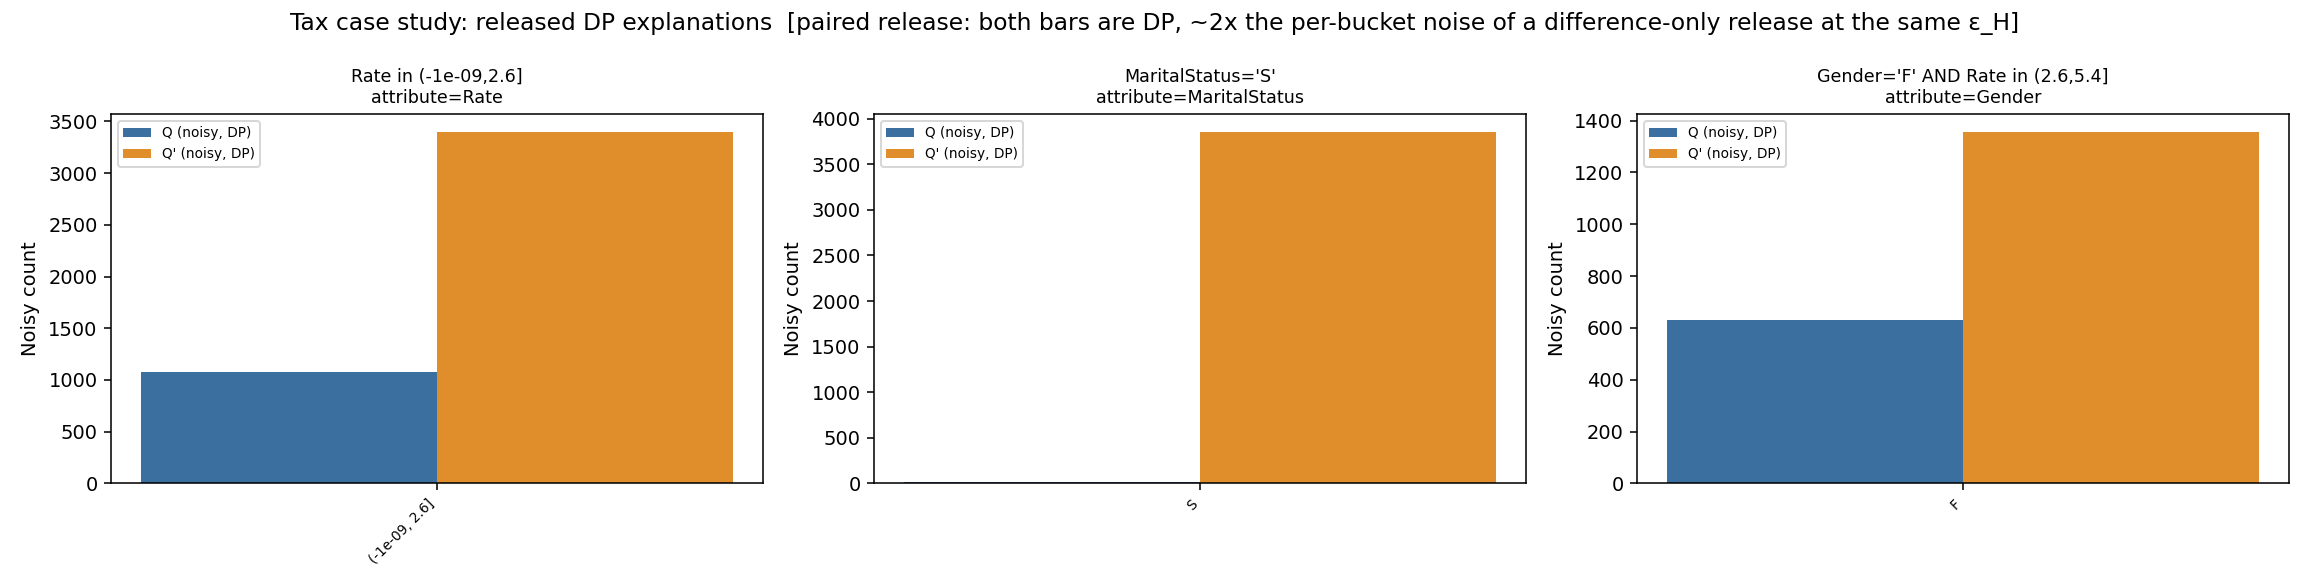
\includegraphics[width=\linewidth]{figures/tax_case_released_histograms_combined.png}
\caption{
Released differentially private histograms for the two most informative
explanations. Negative values indicate buckets that are more frequent in
the refined query result $Q'$ than in the original query result $Q$.
Left: the refinement introduces single taxpayers across low-rate buckets.
Right: the refinement changes the distribution of child-related tax
exemptions among female taxpayers.
}
\label{fig:tax-released-histograms}
\end{figure}

The explanations reveal that the refinement satisfies the representation
constraint primarily by introducing a previously excluded subgroup of
single taxpayers. The released histograms further show that the added
population differs in family-related tax attributes, demonstrating that
the refinement changes both the size and the semantic composition of the
result set. These insights are obtained solely from differentially private
histogram releases.

\subsection{Adult Dataset Case Study}

We next evaluate our framework on the Adult dataset. The original query
selects full-time workers in a specific occupational group:

\begin{verbatim}
SELECT *
FROM Adult
WHERE occupation = 'Craft-repair'
  AND hoursPerWeek >= 40
\end{verbatim}

This query is natural for an analyst interested in full-time craft and
repair workers. However, the result is highly male-dominated and violates
a representation constraint requiring at least 25\% female tuples. The
refinement mechanism broadens the query by removing the occupational
predicate:

\begin{verbatim}
SELECT *
FROM Adult
WHERE hoursPerWeek >= 40
\end{verbatim}

The refined query satisfies the constraint by expanding the result from a
narrow occupational group to the broader population of full-time workers.
Table~\ref{tab:adult-case-study} summarizes representative explanations.

\begin{table}[t]
\centering
\scriptsize
\setlength{\tabcolsep}{3pt}
\renewcommand{\arraystretch}{1.15}
\begin{tabularx}{\linewidth}{p{1.95cm}p{1.45cm}X}
\toprule
Predicate View & Attribute & Interpretation \\
\midrule
\makecell[l]{\texttt{occupation=}\\\texttt{'Tech-support'}}
&
\texttt{occupation}
&
Introduces 1,147 full-time tech-support workers that were excluded by
the original occupation predicate.
\\

\makecell[l]{\texttt{occupation=}\\\texttt{'Other-service'}}
&
\texttt{hours}
&
Adds 2,551 full-time service workers, showing that the refined result is
occupationally broader.
\\

\makecell[l]{\texttt{occupation=}\\\texttt{'Farming-}\\\texttt{fishing'}}
&
\texttt{hours}
&
Introduces 1,197 workers from another manual occupation, with a distinct
working-hours distribution.
\\

\makecell[l]{\texttt{occupation=}\\\texttt{'Farming-}\\\texttt{fishing'}}
&
\texttt{education}
&
Shows that the added farming-fishing population has a different
education profile.
\\
\bottomrule
\end{tabularx}
\caption{Representative explanations returned by the framework for the
Adult case study.}
\label{tab:adult-case-study}
\end{table}

\begin{figure}[t]
\centering
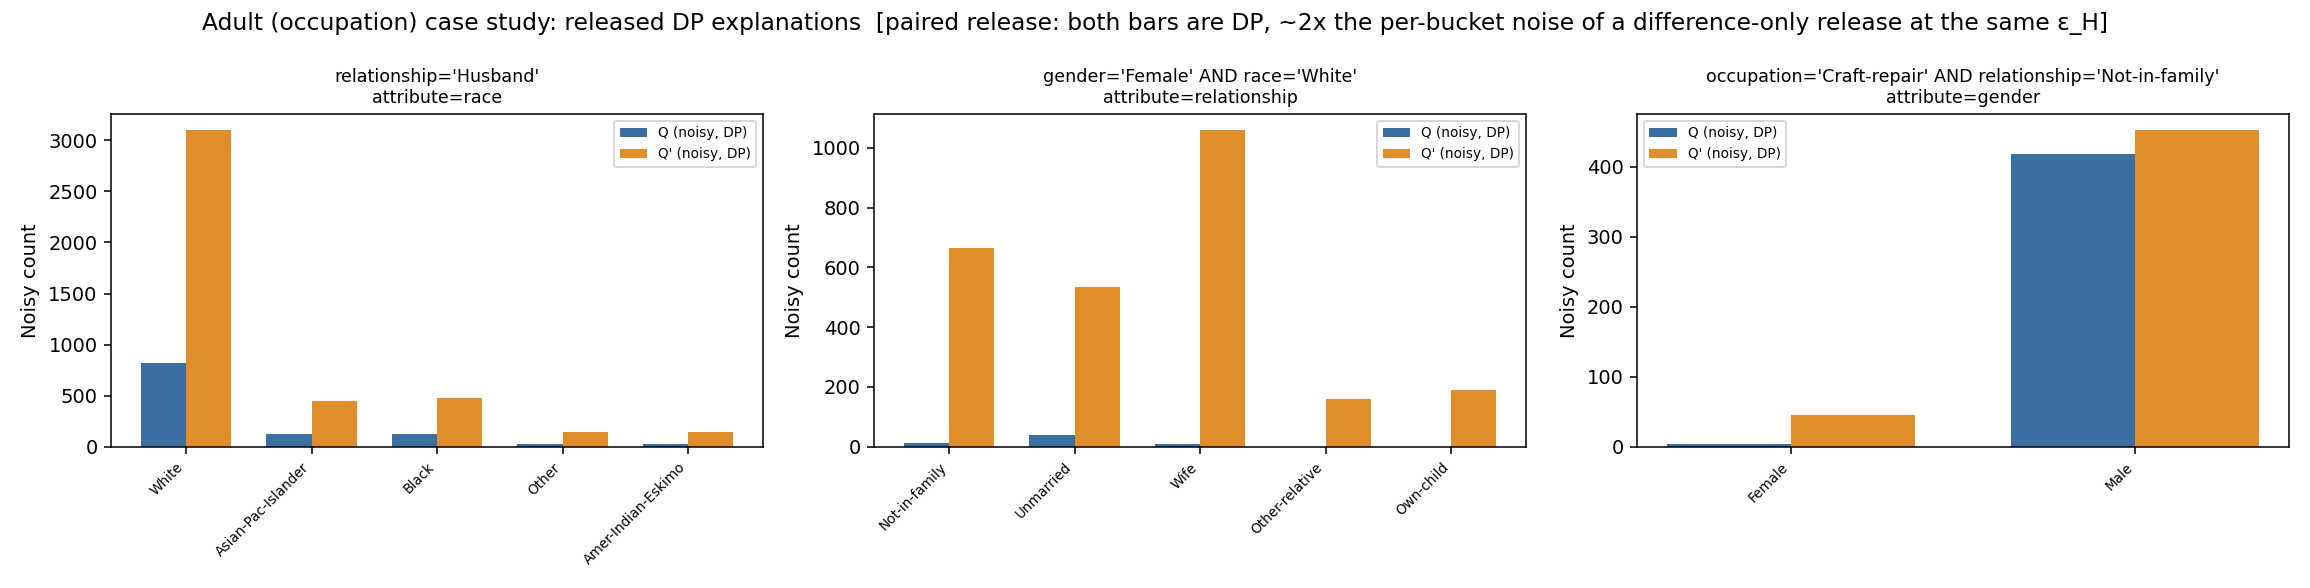
\includegraphics[width=\linewidth]{figures/adult_case_study2_released_histograms_combined.png}
\caption{
Released differentially private histograms for representative
explanations in the Adult case study. Negative values indicate buckets
that are more frequent in the refined query result $Q'$ than in the
original query result $Q$.
}
\label{fig:adult-case-study-histograms}
\end{figure}

The explanations reveal the semantic effect of the refinement. The system
does not simply increase the result size; it admits full-time workers
from occupational groups that were entirely excluded by the original
query, including tech-support, other-service, and farming-fishing workers.
The released histograms further show that the newly added population
differs in both working-hours and education distributions.

% Add to preamble:
% \usepackage{tabularx}
% \usepackage{makecell}
% \usepackage{booktabs}

\subsection{Adult Education--Hours Case Study}

We use the Adult dataset to study a refinement performed in response to
a gender-representation constraint. The original query is:

\begin{verbatim}
SELECT *
FROM Adult
WHERE education IN ('Bachelors','Masters')
  AND hoursPerWeek >= 50
\end{verbatim}

This query selects highly educated workers with intensive work schedules.
However, the result contains only 19.5\% female tuples and therefore
violates the representation constraint requiring at least 25\% female
representation.

To satisfy the constraint, the refinement mechanism produces the
following query:

\begin{verbatim}
SELECT *
FROM Adult
WHERE education = 'Masters'
  AND hoursPerWeek >= 30
\end{verbatim}

The refinement simultaneously restricts the education predicate while
relaxing the working-hours predicate. The refined query increases female
representation to 30.6\%, thereby satisfying the constraint.

The goal of the explanation mechanism is to explain how this refinement
changes the semantic composition of the query result.

\begin{table}[t]
\centering
\scriptsize
\setlength{\tabcolsep}{3pt}
\renewcommand{\arraystretch}{1.15}
\begin{tabularx}{\linewidth}{p{2.2cm}p{1.5cm}X}
\toprule
Predicate View & Attribute & Interpretation \\
\midrule

\makecell[l]{\texttt{relationship=}\\\texttt{'Husband'}}
&
\texttt{occupation}
&
The refinement removes a substantial fraction of executive-managerial,
sales, and craft-repair workers that were overrepresented in the
original result. At the same time, it changes the balance between
managerial and professional occupations.
\\

\makecell[l]{\texttt{relationship=}\\\texttt{'Husband'}}
&
\texttt{income}
&
The refinement removes many high-income workers. This indicates that
satisfying the gender constraint is associated with a noticeable shift
in the economic profile of the selected population.
\\

\makecell[l]{\texttt{race=}\\\texttt{'Asian-Pac-}\\\texttt{Islander'}}
&
\texttt{relationship}
&
The refinement also changes family-relationship composition within this
racial group, although this effect is weaker than the dominant
occupation and income explanations.
\\

\bottomrule
\end{tabularx}
\caption{Representative explanations returned by the framework for the
Adult education--hours case study.}
\label{tab:adult-education-hours}
\end{table}

\begin{figure}[t]
\centering
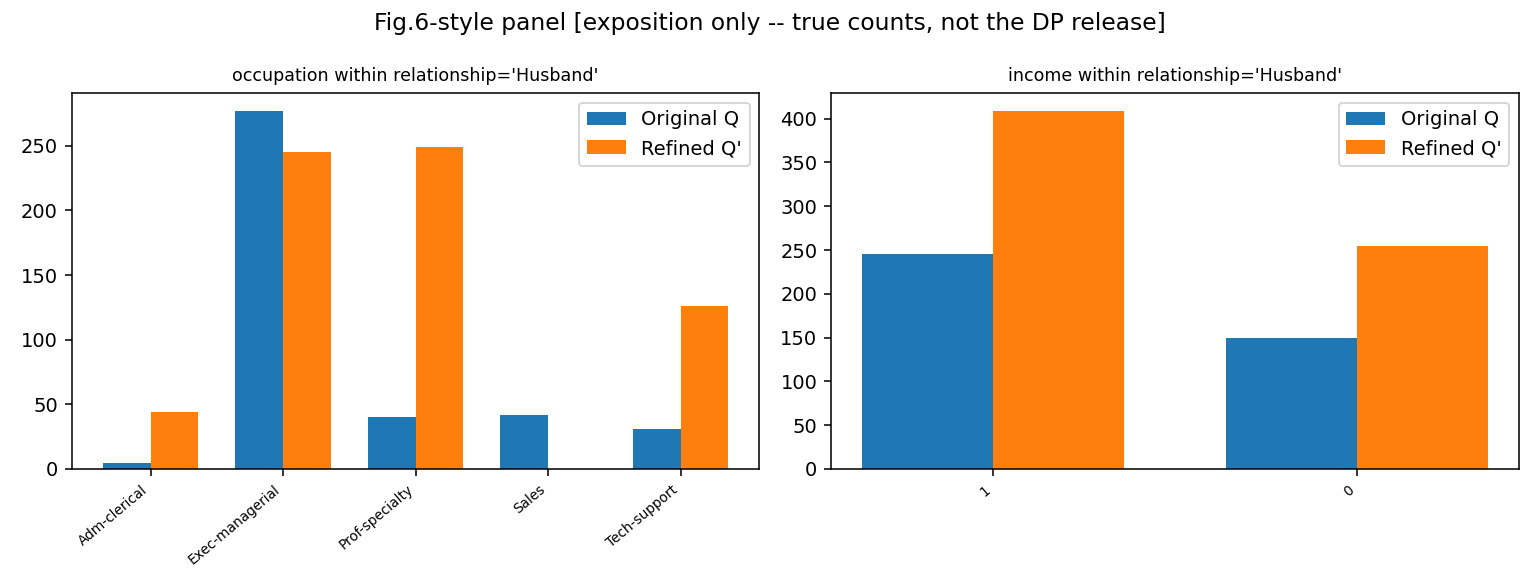
\includegraphics[width=\linewidth]{figures/adult_education_hours_combined_vldb_ready.png}
\caption{
Differentially private explanations for the Adult Education--Hours
case study. (a) Occupation distributions within the view
\texttt{relationship='Husband'} for the original query $Q$
and the refined query $Q'$. The refined query substantially
changes the occupational composition of the selected population.
(b) Income distributions for the same view, showing a corresponding
shift in economic characteristics. Together, the explanations
reveal that satisfying the gender-representation constraint is
associated with broader occupational and income changes rather
than merely increasing the number of female tuples.
}

\label{fig:adult-education-hours}
\end{figure}

The explanations reveal that the refinement does not satisfy the gender
constraint by directly manipulating gender. Instead, it replaces a
population of highly educated workers with long working hours by a more
specialized population of Master's-degree holders who work fewer hours.
This change indirectly increases female representation.

The released histograms show that the refined query excludes many
high-income managerial and sales workers who were overrepresented in the
original result. Consequently, the refinement introduces a trade-off:
improving gender representation comes at the cost of altering both the
occupational and economic composition of the selected population.

This case study demonstrates how our framework helps users understand
not only whether a refinement satisfies a representation constraint, but
also which semantic changes were responsible for achieving that goal.

\subsection{Quality Measures}
\label{subsec:quality-measures}

We evaluate the quality of the explanations using the following measures.

\paragraph{Score approximation.}
We compare the utility score of the explanations selected by the private method
against the best non-private score:
\[
    \mathrm{ApproxRatio}
    =
    \frac{\mathrm{score}(E_{\mathrm{private}})}
         {\mathrm{score}(E_{\mathrm{nonprivate}})}.
\]

\paragraph{Rank of selected explanations.}
For each explanation selected by the private method, we compute its rank in the
non-private ordering of all candidate explanations.

\paragraph{Histogram error.}
We measure the error introduced by the Laplace mechanism using the $L_1$ distance
between the released noisy histogram and the corresponding non-private histogram:
\[
    \mathrm{HistErr}(\widehat{H}, H)
    =
    \sum_{v \in \mathrm{Dom}(A)} |\widehat{H}(v) - H(v)|.
\]

\paragraph{Stability across trials.}
We measure how often the same explanation attributes and predicates are selected
across repeated runs with the same parameter configuration.

% TODO: Decide which quality measures will appear in the final paper.
% TODO: Add plots for score approximation, rank, histogram error, and stability.

\subsection{Implementation Details}
\label{subsec:implementation-details}

All experiments are implemented in \textbf{\texttt{TODO: Python version / framework}}
and executed on \textbf{\texttt{TODO: machine specs}}.

Each experiment is represented as a configuration object containing:
\begin{itemize}
    \item date and time;
    \item description;
    \item dataset;
    \item query pair;
    \item constraints;
    \item refinement algorithm;
    \item $k$;
    \item $\epsilon$;
    \item $\tau$;
    \item predicate-generation configuration;
    \item number of trials.
\end{itemize}

% TODO: Add a short description of the experiment framework classes:
% BaseExperiment, Dataset, Query, Condition, Constraint, DemographicGroup,
% Attribute, AttrType, Operator.

\subsection{Summary of Findings}
\label{subsec:experiments-summary}

% TODO: Fill this subsection after running the experiments.

The experimental results show that \textbf{\texttt{TODO: main scalability finding}}.
They also show that \textbf{\texttt{TODO: main quality finding}}. Finally, the case
studies demonstrate that \textbf{\texttt{TODO: main interpretability finding}}.
